\section{\system Overview}\label{sec:overview}
\system is a staging compiler for Python.
The runtime provides a \texttt{CoyoteVar} datatype which represents a symbolic encrypted value, and supports addition, subtraction, and multiplication.
Python code that manipulates these symbolic variables produces an arithmetic circuit representation of the program, which \system then compiles into a set of vector primitives that can be further lowered into C++ code that targets Microsoft's SEAL backend for BFV \raghav{(citation needed)}.

% \milind{You should put the step-by-step procedure for coyote here, then describe them in more detail: break the computation down into aligned subgraphs, assigning scheduling slots, choosing lanes. This is also a good place for a picture explaining these steps: show a tree, show picking bits of a tree, show moving when the computations happen around, show lane assignment}

% \milind{This whole section will benefit from having a running example :-)}
 
\subsection*{Compilation Steps}
\begin{figure}
    \begin{subfigure}{0.45\columnwidth}
        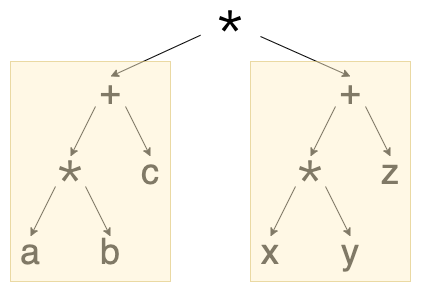
\includegraphics[scale=0.25]{figures/compilation_overview/small_expression_circuit.drawio.png}
        \caption{Arithmetic circuit computing $$(ab+c)(xy+z)$$ with vectorizable subcircuits highlighted}
        \label{fig:small-expr-circuit}
    \end{subfigure}
    \begin{subfigure}{0.45\columnwidth}
        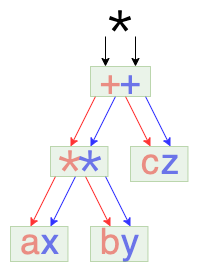
\includegraphics[scale=0.4]{figures/compilation_overview/stacked_vector_circuit.drawio.png}
        \caption{Arithmetic circuit with highlighted subcircuits vectorized}
        \label{fig:partially-vectorized-circuit}
    \end{subfigure}
    \begin{subfigure}{0.3\columnwidth}
        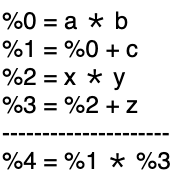
\includegraphics[scale=0.3]{figures/compilation_overview/code_split_into_phases.drawio.png}
        \caption{Scalar code split into vectorizable epochs}
        \label{fig:code-split-epochs}
    \end{subfigure}
    \begin{subfigure}{0.6\columnwidth}
        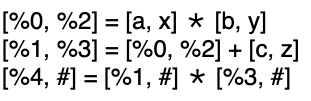
\includegraphics[scale=0.3]{figures/compilation_overview/vector_schedule_needing_rotates.drawio.png}
        \caption{Vector schedule for scalar code demonstrating need for rotation}
        \label{fig:vector-sched-needing-rotates}
    \end{subfigure}
    \caption{A running example of how \system vectorizes arbitrary arithmetic circuits}
    \label{fig:toy-running-example}
\end{figure}

In this section, we give a brief overview of the steps \system takes to vectorize an arbitrary arithmetic circuit.
We will use the circuit in Figure~\ref{fig:small-expr-circuit} that computes $(ab+c)(xy+z)$ as a running example.
The compilation proceeds as follows:
\begin{enumerate}
    \item \system first identifies highly vectorizable subcircuits (shown highlighted in Figure~\ref{fig:small-expr-circuit})
    \item These subcircuits are pulled out and aligned to produce a single vectorized computation, \milind{Mention here that the key challenge is figuring out which computations can be grouped together into vector operations, and which input data should be put into vector ``registers.''} which is then inserted back into the original program, resulting in the circuit in Figure~\ref{fig:partially-vectorized-circuit}. 
    This process amounts to essentially precomputing part of the program, \milind{This is confusing. I don't know in what way it represents precomputing part of the program. Why not just say that this step produces a vectorized subcircuit and lave it at that?} and is repeated until no more subcircuits can be found. 
    At this point, the scalar computation has been split into multiple {\em epochs},\milind{Maybe emphasize here that each subcircuit creates an epoch} as seen in Figure~\ref{fig:code-split-epochs}, and each epoch has been vectorized separately. \milind{Mention here that the key challenge is that the outputs of one epoch are consumed by another epoch, and the outputs need to be in the right spot so that the next epoch can consume them.}
    \item The new circuit is converted to a vector {\em schedule} (Figure~\ref{fig:vector-sched-needing-rotates}), which amounts to assigning a {\em lane} (horizontal position) and {\em schedule slot} (vertical position) to each original scalar instruction.
    \item \milind{This ``notice'' is part of the previous item :-)} Notice that in the schedule, the scalar \texttt{\%3} is computed on lane 2, but used in lane 1. To correct this discrepancy, \system inserts an additional instruction to create a copy of the \texttt{[\%1, \%3]} vector with data arranged as \texttt{[\%3, \%1]}, putting \texttt{\%3} on lane 1 where it is used.
\end{enumerate}

% enumerate
% add figure
% \milind{This dives in too quickly; I think the overview thing I laid out above is necessary. Otherwise: what's a stage? What does it mean to schedule subgraphs together? What does it mean to ``line operands up.''}
\raghav{Is this better? I kind of briefly mentioned ``creating a vector schedule'' as a separate thing that needs to happen apart from just picking vectorizable trees, should I say any more or less about that here, before discussing it in detail in Section~\ref{sec:design}?}
% \system reduces the search space for vectorized programs \raghav{Does it make sense to call it ``search space''?} by first splitting the computation into multiple stages, and only allowing for vector rotations to line operands up between stages.
% A stage consists of a set of independent subgraphs of the entire circuit \raghav{Do I need to explain what independent means here?}. 
% The subgraphs are scheduled together, with each one being placed on its own vector lane. 
% Once vector code for a stage has been generated, all of its subgraphs are removed from the circuit, and the subgraphs for the next stage are picked out.
% After the entire circuit has been split up into stages, the subgraphs from each stage are assigned specific vector lanes to minimize the number of distinct rotations required to line up the outputs of one stage with the inputs of the next.
% Finally, \system computes and inserts these rotation instructions between stages and emits the vector code.

\subsection{Backend}\raghav{What more can/should I say here? Is this the right place to mention why we don't use CKKS (cost model constraints)? Is that even relevant to mention?} \milind{Say something about how security parameters are chosen? Add a footnote saying that we target BFV instead of CKKS because the cost model is more amenable to general vectorization. It's not a major point, but it's worth mentioning to preempt reviewer questions.}
\system targets the BFV backend for Microsoft SEAL \raghav{(citation needed)}.